\begin{problem}{슈퍼컴퓨터}
	{standard input}{standard output}
	{3 seconds}{128 megabytes}{}
	
	범수는 새로운 구조의 슈퍼컴퓨터를 개발했다. 이 슈퍼 컴퓨터는 같은 종류의 처리장치 여럿으로 이루어져 있다. 하나의 처리장치는 1 단위시간에 하나의 명령을 실행할 수 있다.
	
	이 컴퓨터용 프로그램은, 순차적인 실행이 아니라 트리모양의 구조를 가지고 있다. 하나의 명령은 0개, 1개 또는 2개 이상의 \textit{후속명령}을 가질 수 있다. $a$가 $b$의 후속명령이면, $b$는 $a$의 \textit{부모명령}이다.
	
	프로그램의 명령들은 병렬처리가 될 수 있다. 그리고, 다양한 순서로 실행될 수 있다. 단 하나의 제약조건은, 어떤 명령은 그 부모명령이 실행되기 전에는 실행될 수 없다는 것이다. 예를 들어, 한 명령의 후속 명령들은 어떠한 순서로도 병렬로 실행될 수 있다.
	
	범수는 실행해야할 어떤 프로그램이 있다. 범수는 그의 자원을 효율적으로 사용하는 것을 좋아하기 때문에, 처리장치의 갯수가 프로그램의 실행에 어떠한 영향을 미칠지 궁금해 졌다. 그는 프로그램과 처리장치의 갯수가 주어졌을 때, 슈퍼컴퓨터로 프로그램을 실행하는 최소시간을 구하고 싶어 한다.
	
	\InputFile
	
	첫째 줄에는 범수의 프로그램의 명령어 수를 의미하는 $n$과 쿼리 갯수를 의미하는 $q$가 공백 하나로 구분되어 주어진다. ($1 \le n, q \le 1,000,000$) 
	
	둘째 줄에는 $q$개의 정수 $k_1, k_2, \cdots, k_q$가 공백 하나로 구분되어 주어진다. ($1 \le k_i \le 1,000,000$) $k_i$는 범수의 $i$번째 쿼리를 의미한다.
	
	마지막 줄인 세번째 줄에는 $n-1$개의 수열 $a_2, a_3, \cdots, a_n$이 공백 하나로 구분되어 주어진다. ($1 \le a_i < i$) $a_i$번 명령은 $i$번 명령의 부모명령이다. 명령은 1부터 $n$까지 번호가 붙어있고, 1번 명령은 프로그램의 가장 처음 명령이다.
	
	
	\OutputFile
	
	프로그램은 $q$개의 정수가 공백 하나로 구분된 한 줄을 출력해야 한다. $i$번째 수는 $k_i$개의 처리장치로 이루어진 슈퍼컴퓨터가 명령을 실행하는데 걸리는 최소시간을 출력해야 한다.	
	
	\SubtaskWithCost{1}{20}
	\begin{itemize}
		\item $n \le 1,000$
		\item $q \le 10$
	\end{itemize}
	
	\SubtaskWithCost{2}{15}
	\begin{itemize}
		\item $n \le 30, 000$
		\item $q \le 50$
	\end{itemize}
	
	\SubtaskWithCost{3}{65}
	
	추가 제한조건이 없다.
	
	\Examples
		
	\begin{example}
	\exmp{
20 1
3
1 1 1 3 4 3 2 8 6 9 10 12 12 13 14 11 11 11 11
	}{%
8
	}%
	\end{example}
	
	\Notes
	
	\begin{center}
		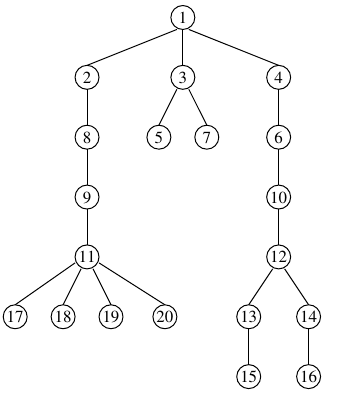
\includegraphics[]{sup.png}
	\end{center}
	
	프로그램 명령은 다음과 같은 순서로 실행될 수 있다.
	
	\begin{center}
	
	\begin{tabular}{|r|rrr|}
		\hline
		\multicolumn{1}{|c|}{\large \textbf{시간}}& \multicolumn{3}{c|}{\large \textbf{명령}} \\ \hline
		1&      1&       &       \\ 
		2&      2&      3&     4 \\ 
		3&      5&      6&     7 \\ 
		4&      8&     10&       \\ 
		5&      9&     12&       \\ 
		6&     11&     13&    14 \\ 
		7&     15&     16&    17 \\ 
		8&     18&     19&    20 \\ \cline{1-4}
	\end{tabular}
	\end{center}
	
\end{problem}

